% !TEX root = main.tex

\chapter{試料構造と測定方法}%================================
\section{はじめに}%========================================
本研究ではInGaAs/GaAs系多重量子井戸・ファブリーペロー型の半導体レーザーをデザインし測定を行った。本章では2.2節でそのエピ構造とデバイス化のためのプロセスについて、2.3節で測定手法について述べる。
\section{試料作製}%========================================
本研究ではInGaAs/GaAs系3周期歪量子井戸レーザーおよびInGaAs/GaAsP系10周期歪補償量子井戸レーザーを作製したした。本2.2節では結晶構造のデザインと測定するためのデバイス化について述べる。エピウエハのデザインおよび結晶成長、フォトリソグラフィー加工に関してはNTT-AT社、オプトウェル社に委託し試料を作製していただいた。この場をお借りして感謝を表する。

\subsection{試料構造}%=====================================
まずはエピウエハ構造について述べる。本研究では2種類の試料を作製した。\\
(1)InGaAs/GaAs系3周期歪量子井戸構造\\
(2)InGaAs/GaAsP系10周期歪補償量子井戸構造\\
である。それぞれのエピ構造を図\ref{fig:fig_2_1_wafer_structure}に示す。
下からnタイプGaAs基板、nタイプAlGaAsクラッド層、non-GaAs SCH層(Separate Confinement Hetero-Structure)、活性層、non-GaAs SCH層、p-InGaPエッチングストップ層、p-GaAs層、p-AlGaAsクラッド層、p-GaAsハイドープコンタクト層となっている。
バンドギャップの話して発光領域の話
活性層には(1)3周期多重量子井戸のエピウエハでは量子井戸層を$\rm{In_{0.255}Ga_{0.745}As}$、バリア層をGaAsを用いた。GaAs基板に格子整合を行った。$\rm{In_{1-x}Ga_{x}As_{y}P_{1-y}}$4元混晶の格子定数はべガードの法則
\begin{eqnarray}
a(x,y)=5.8687-0.4176x+0.1896y+0.0125xy
\end{eqnarray}
で求められる\cite{ref_iga}。これより$\rm{In_{0.255}Ga_{0.745}As}$活性層の格子定数は5.7565\AA 。GaAsバリア層の格子定数は5.6532\AA であるので、面内歪$-\Delta a/a=$は-0.0183 となる。InGaAs層に圧縮歪が生じている。(2)10周期量子井戸のエピウエハにおいては量子井戸層を同様に$\rm{In_{0.255}Ga_{0.745}As}$、バリア層では歪補償のために$\rm{GaAs_{0.71}P_{0.29}}$を用い、GaAs基板に格子整合を行った。(GaAsPのGaAsに対する歪は$-\Delta a/a=0.010$でありGaAsPには引っ張り歪が生じている)

また図\ref{fig:fig_2_1_wafer_structure}にはバンドギャップ$E_{g}$と屈折率nの変化を模式的に表した。光は活性層とSCH層、p-InGaAs層、p-GaAs層に閉じ込められると考えいている。またキャリアは$E_{g}$の小さい量子井戸へ流れ込む。量子井戸で再結合がおこる。

エピウエハ完成後フォトリソグラフィによって電極パターンを形成した。それについて次節で述べていく。
\begin{figure}[h]
	\centering
	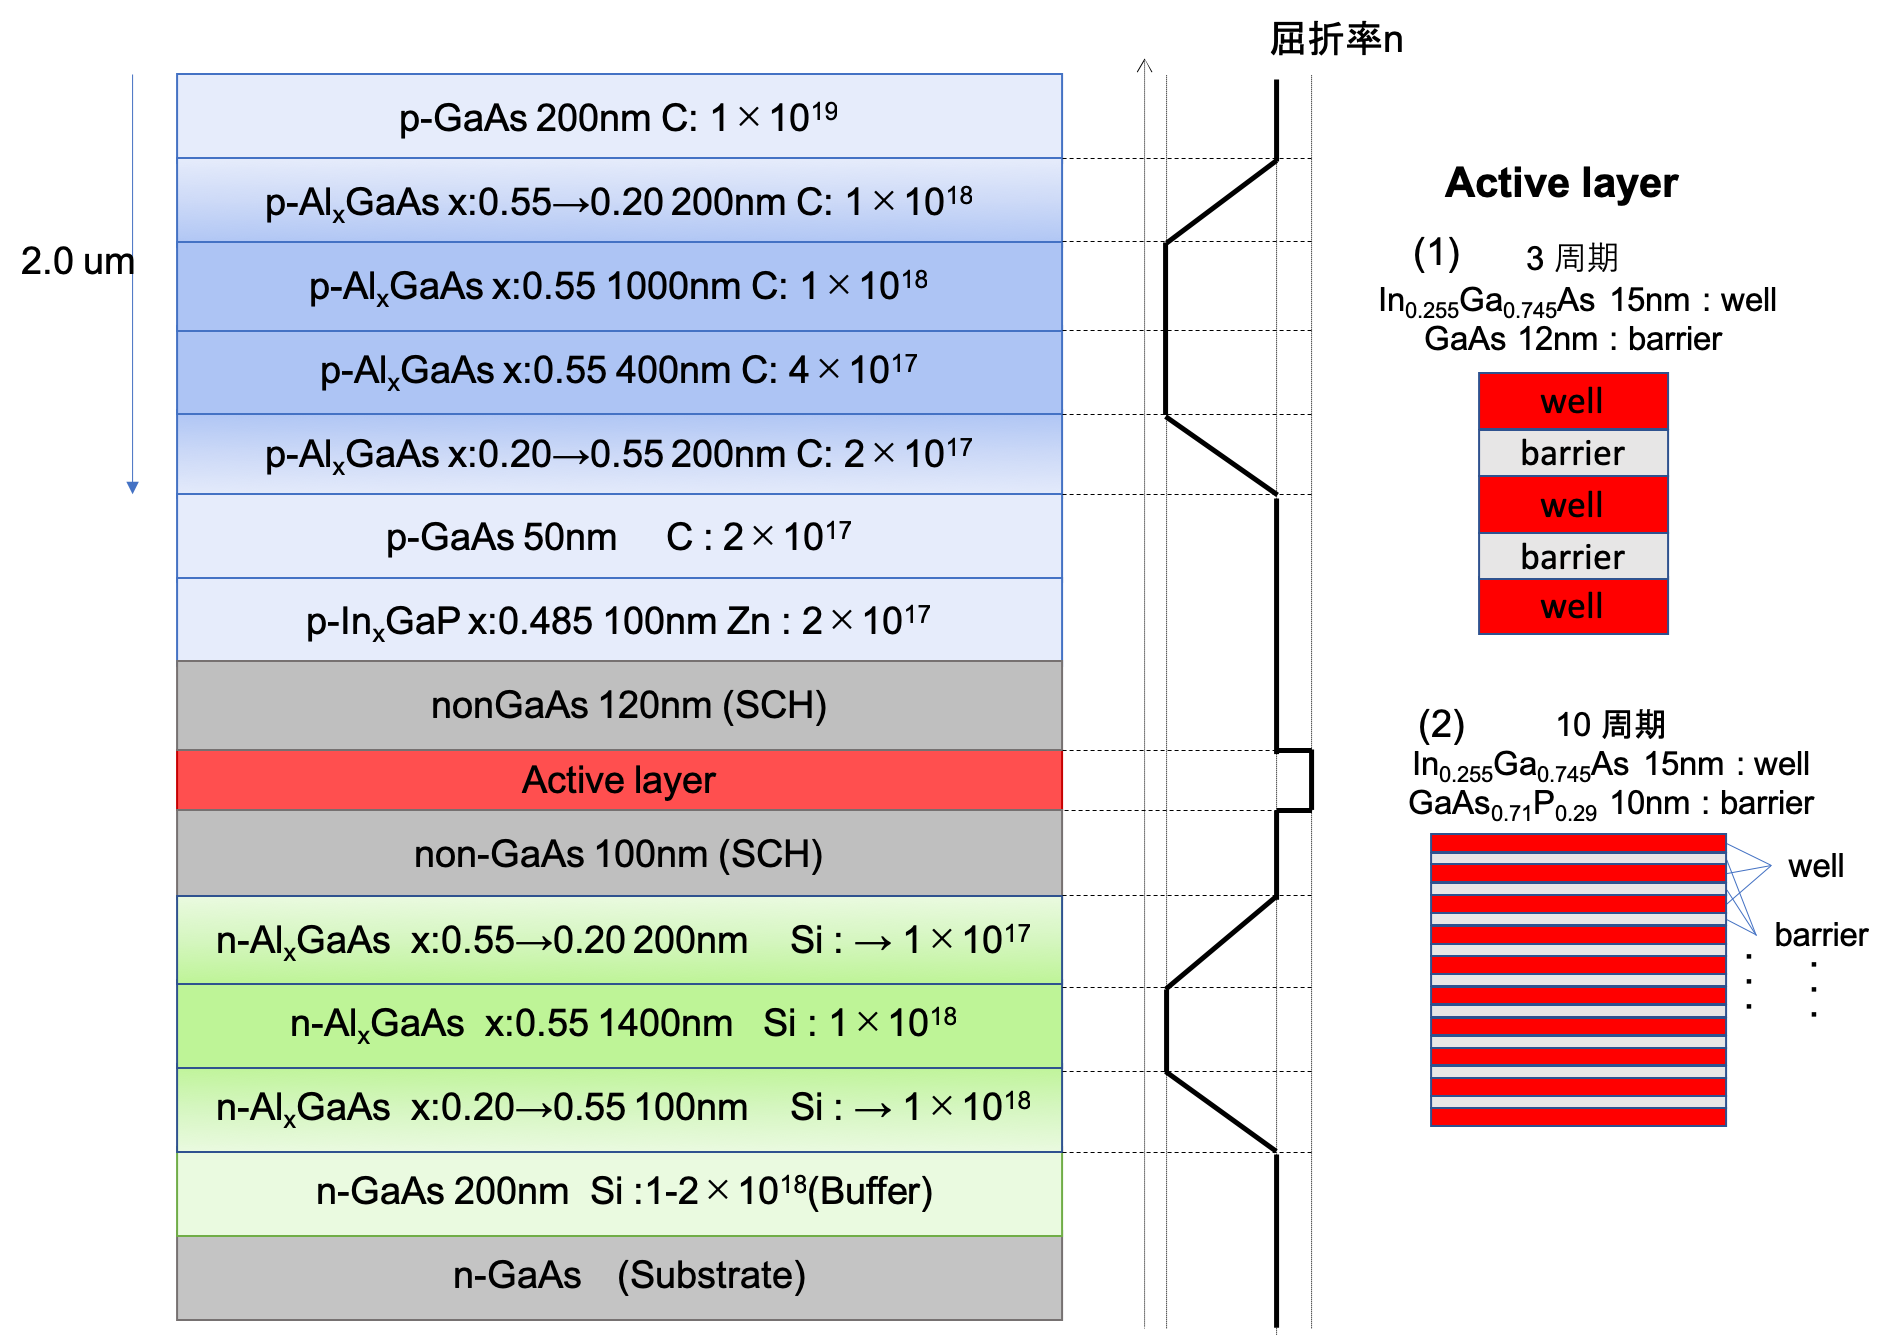
\includegraphics[width=10cm]{figure/fig_2_1_wafer_structure}
	\caption{エピウエハ構造}
	\label{fig:fig_2_1_wafer_structure}
\end{figure}
%\clearpage
\subsection{ブロードコンタクトレーザー}%=======================
ブロードコンタクトレーザーとは光導波路を形成せずコンタクト電極をベタに蒸着したレーザーデバイスである。リッジ形成プロセスを簡略化することで早く測定を行うことを目的とした。ウエハの評価測定のために用いた。
エピウエハのn側とp側にコンタクトメタルの蒸着を行った。p側の原子はAuZnNiをコンタクトメタルとしTi/AuおよびAu電極を使用した。基板を研磨し120um厚とした。その後n側はAuGeNiを用いて電極を蒸着した。


劈開を行いレーザーデバイス化した後の模式図を図\ref{fig:sample_broadcontact}に示す。z方向にファブリーペロー共振器が形成される。y方向に電流が流れ、活性層でキャリアの再結合が起きる。赤い楕円で示した。注入キャリアの量が閾値を超えると反転分布となり誘導放出がおこる。光が共振器内部を往復することで増幅され発振に至る。

共振器長はL=500,1000,2000umの3種類を作製した。
x方向の電流の広がりの大きさを定める電極の幅を「電極パッド幅w」と呼ぶことにする。電極パッド幅はw=3,5,10,30,50,100,300umの6種類を作製した。

\begin{figure}[t]
	\centering
	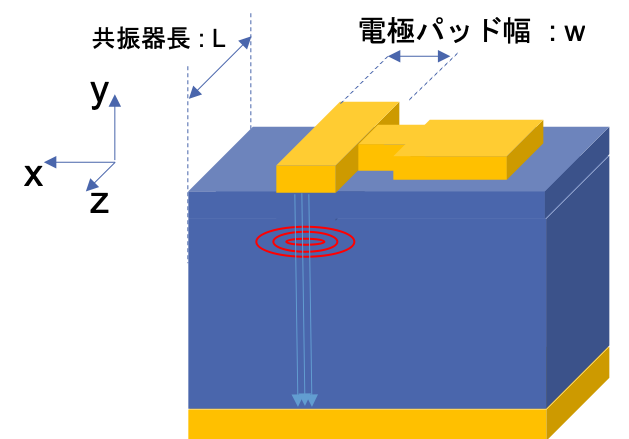
\includegraphics[width=10cm]{figure/fig_2_1_broadcontact.png}
	\caption{ブロードコンタクレーザー}
	\label{fig:sample_broadcontact}
\end{figure}

\begin{comment}
\begin{figure}[t]
	\centering
	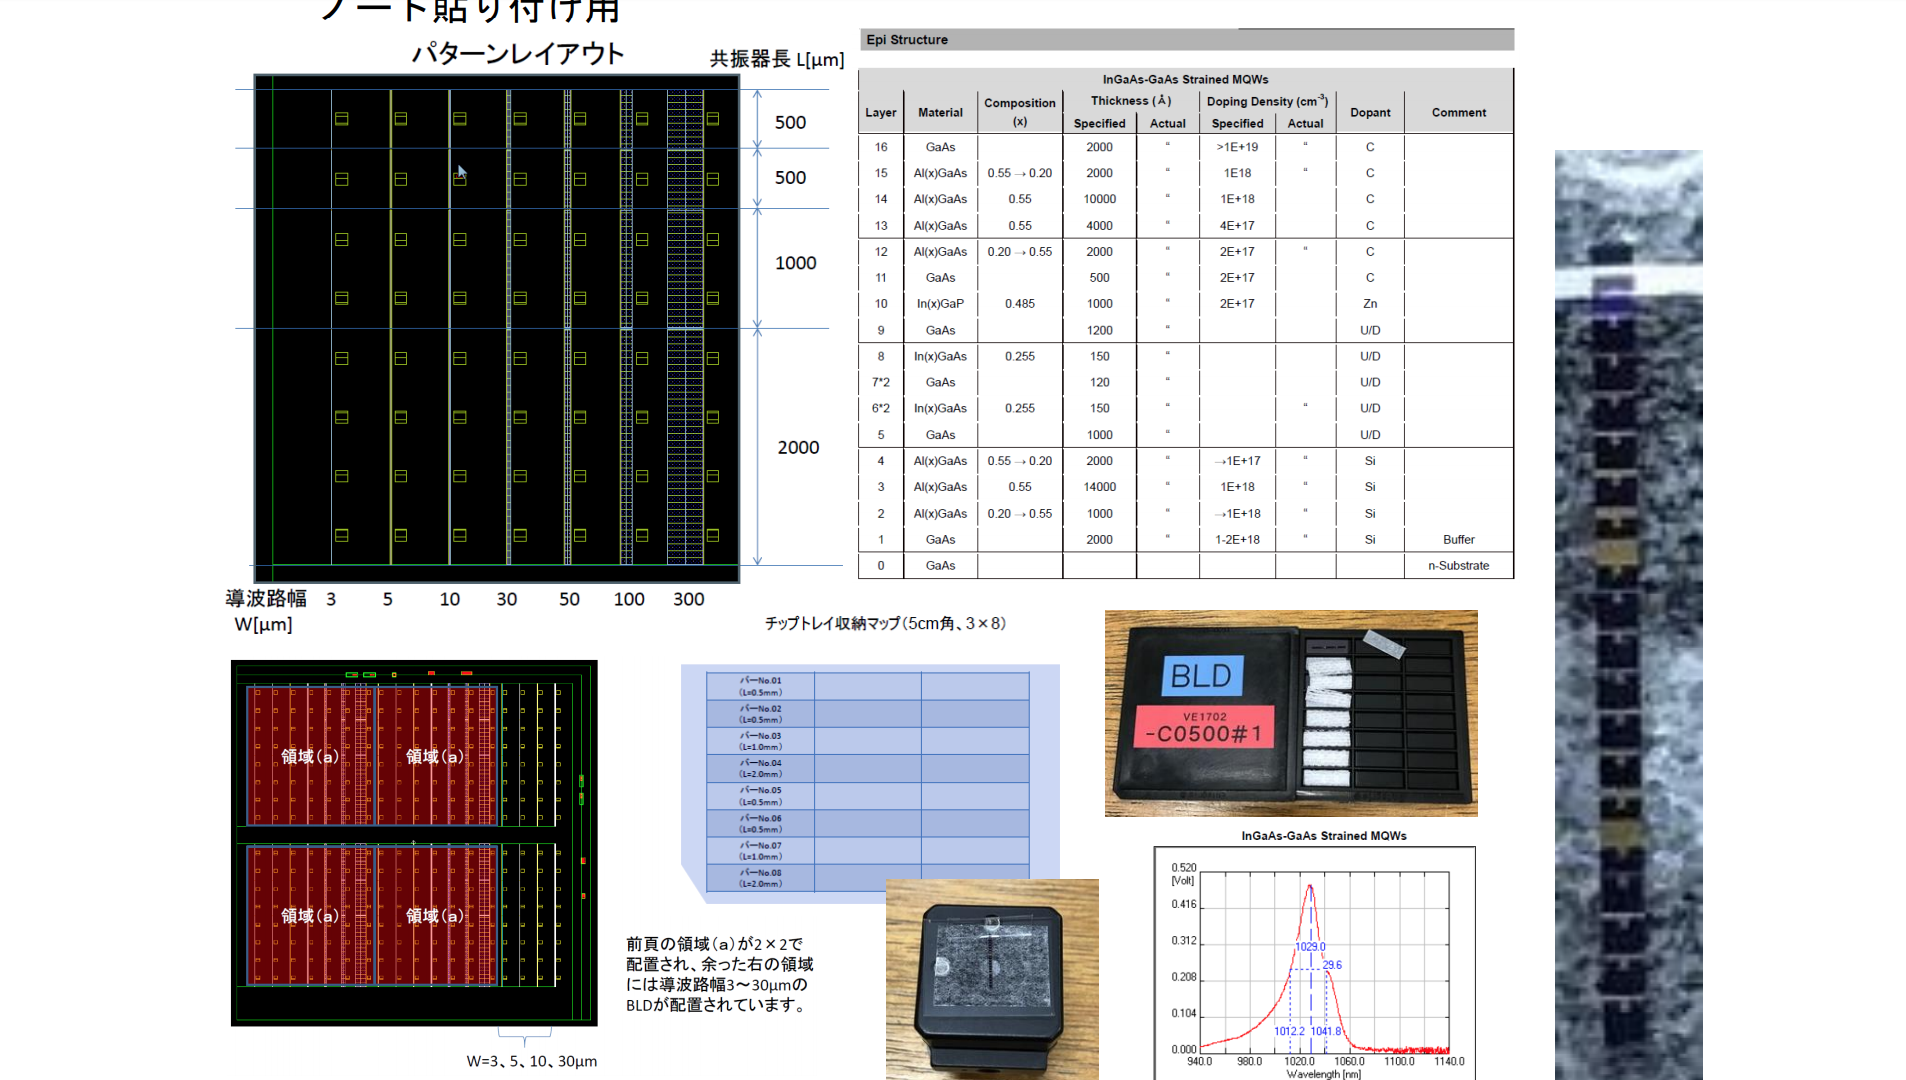
\includegraphics[width=10cm]{figure/fig_2_1_broadcontact_memo.png}
	\caption{ブロードコンタクレーザーめも}
	\label{fig:sample_broadcontact_memo}
\end{figure}
\end{comment}
\subsection{リッジ導波路型レーザー}%==========================
次にリッジ導波路型レーザーについて述べる。その模式図を図\ref{fig_2_1_ridge}に示す。エピウエハ作製後p側クラッド層をy方向に活性層直上までエッチングすることで光導波路を形成した。そのときx方向のリッジ幅をwと呼ぶ。x方向の光閉じ込めが大きくなるため、キャリアと光の重なりが大きくなることにより利得を大きくすることができる。%参考文献ほしい
商用デバイスにおいても一般的に行われている手法である。本研究でも最終的に利得スイッチング動作を試みるデバイスである。


導波路リッジの深さは3周期試料は実測値で1.8um、10周期試料は1.9$\sim$2.0umである。導波路リッジ幅はw=1.5um,2.5umのものを作製した。
AuZnNiをコンタクトメタルとしてTi/Auを電極とした。
基板を研磨し120um厚とした。n側コンタクトはAuGeNi/Auである。
共振器長L=100,200,300,400,500,1000umに劈開を行った。共振器長が100,200umのものは劈開の真っ直ぐさを保つために60um厚と非常に薄く研磨した。
\begin{figure}[t]
	\centering
	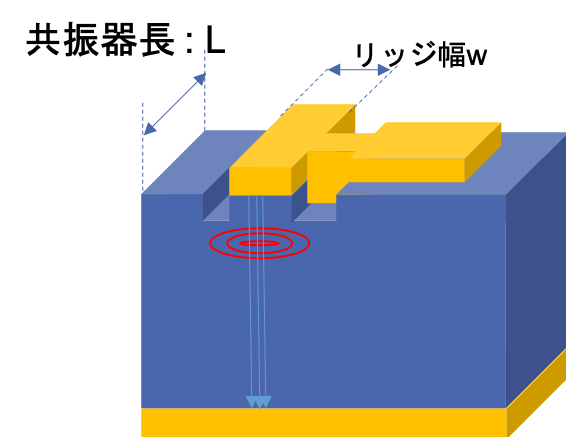
\includegraphics[width=10cm]{figure/fig_2_1_ridge.png}
	\caption{リッジ導波路型レーザー}
	\label{fig_2_1_ridge}
\end{figure}
\clearpage
\subsection{マウント}%======================
作製したブロードコンタクトレーザーおよびリッジ導波路型レーザーに電流注入実験を行うためにマウントを行なった。

定常電流を流す実験を行うためにマウントした試料の例を図\ref{fig:fig_2_1_mount}(a)に示す。写真中心の青い棒状のものがレーザーデバイス(レーザーバー)であり、合計5つの異なる電極パッドがついている。z方向の共振器長は300umである。誘導放出光はz方向に放射する。
 レーザーはAlN基板の全面にAnSnメッキを施したサブマウント(京セラ社製)にダイボンディングを行った。ダイボンディングはAnSuの融点よりも高い330℃まで加熱したサブマウントの上にレーザーバーを吸引ピンセットでおいた。レーザの端面をAlNサブマウントの淵に合わせることが後の測定で光検出器を近づけるために大事である。このときAnSuの酸化を防ぐために$N_{2}$雰囲気下で行った。
電流注入は電極をプローバーで触ることにより行った。
%ブロードコンタクトレーザーはダイボンディングしてなかったっけ?そういえば
この状態で試料上面のp側電極をプローバー
%(先端の径...程度の金属の針)
でさわり電流を流した。n側はAuSnメッキAlNサブマウントを銅板などの導体に置き、その銅板から配線を行った。1本のレーザーバーに5から6個程度の電極素子があるため1つの素子に対して測定が終わると次々とプローバーさわる箇所をかえていった。そうすることで速やかに測定を続けることができる。


 一方、利得スイッチング動作実験(高周波電気パルスを駆動)を行う試料は短い電気パルスが入るようにTransistor Outlineパッケージと呼ばれる缶状の金属にマウントを行った。京セラ社製のCANを用いた。1つ1つに分離した素子をAnSn共晶材あるいはエポキシを用いてTO-CANにダイボンディングし、金線をワイヤーボンディングマシンで配線した。その例を図\ref{fig:fig_2_1_mount}(b)に示す。図\ref{fig:fig_2_1_mount}(b)
a
\begin{figure}[h]
	\centering
	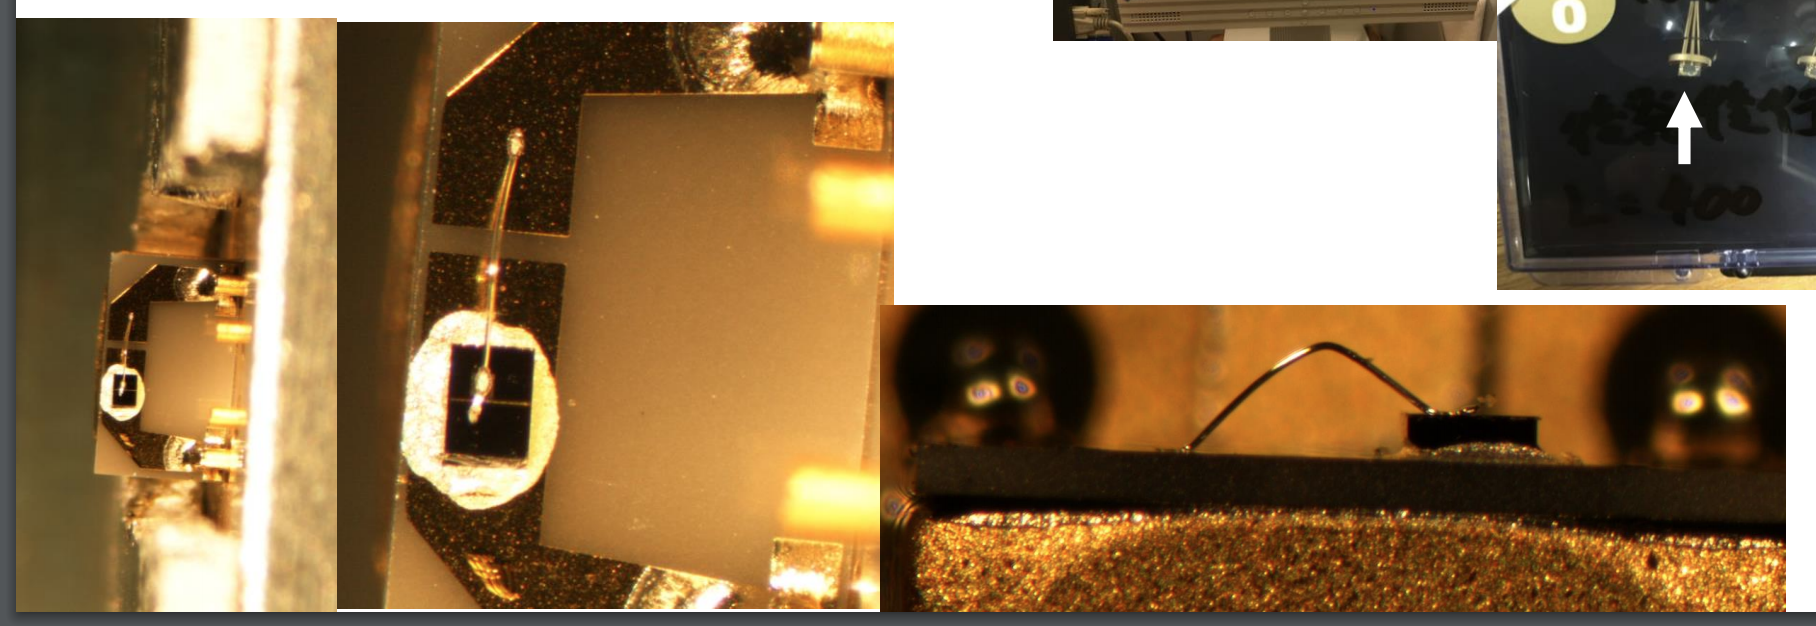
\includegraphics[width=15cm]{figure/fig_2_1_mount.png}
	\caption{測定デバイス外観}
	\label{fig:fig_2_1_mount}
\end{figure}
\clearpage
\section{測定方法}%========================================
本研究では主に2つの実験を行った。1つはエピウエハの品質を評価するための定常電流を印加する実験である。もう一つは利得スイッチング動作を起こすための短い電気パルスを印加する実験である。それぞれについて2.3.1節と2.3.2節で述べる。
\subsection{定常電流注入による測定実験}%=======================
まずエピウエハの品質を調べるために定常電流を注入する実験である。発振閾値電流や発振時の発光効率すなわち外部量子効率などの基本的な物性パラメータを見積もることができる。
実験系を図\ref{fig:fig_2_2_IL_setup}に示す。パルスジェネレータから数usパルスを数ms繰り返し周期で発生させ試料に注入する。ここでマイクロ秒程度のパルスは試料の中での発光過程やその他の物理現象の時間オーダーに対して十分長く、定常電流とみなすことができる。DC電流では熱の影響が大きくなってしまい試料が壊れてしまう恐れがあるため。Duty比(パルス幅と繰り返し周期の比)を1:1000程度に設定して実験を行った。試料からの発光強度を光パワーメータで測定した。また、回路に試料と直列に抵抗(22.4$\rm{\Omega}$)を入れ、そこにかかる電圧をモニタすることで流れる電流をそくていした。また回路全体の電圧と抵抗にかかる電圧の差をとることで試料にかかる電圧を算出した。

本来であればDC電流を印可することで定常発振させることが望ましい。しかし試料への熱の影響が無視できないほど大きくなってしまうため、本研究ではDC電流の代わりにマイクロ秒程度パルス電圧を印可した。マイクロ秒は半導体素子の中が定常状態になるには十分長く印可している時間の間に定常発振が起きているものとみなしていること。

\begin{figure}[htbp]
	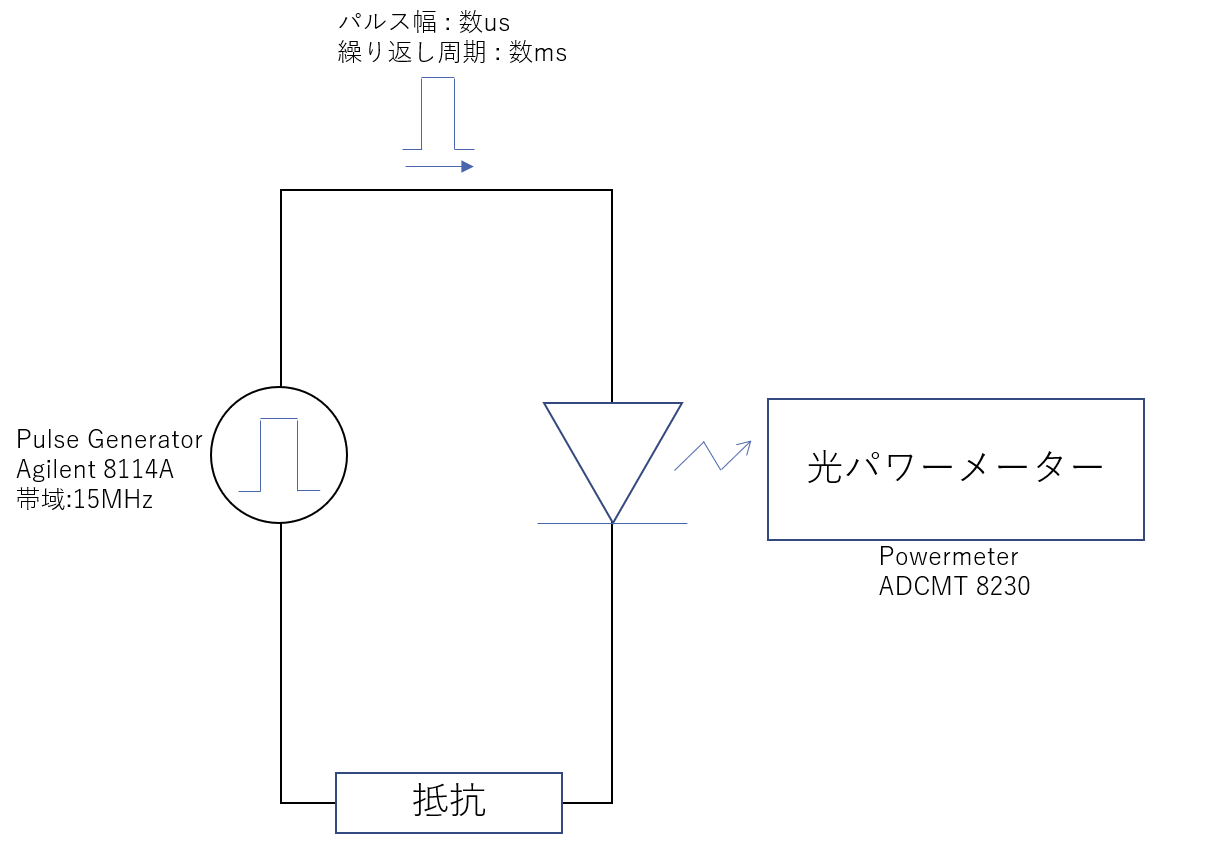
\includegraphics[width=15cm]{figure/fig_2_2_IL_setup.png}
	\caption{定常電流注入実験の実験系回路図}
	\label{fig:fig_2_2_IL_setup}
\end{figure}
\clearpage
ここで用いた機材を\ref{table:table_2_2_IL_setup}に示す。
\begin{table}[hbtp]
  \caption{定常電流印加実験に用いた機材}
    \label{table:table_2_2_IL_setup}
  \centering
  \begin{tabular}{lcr}
    \hline
    機材  & 型番     \\
    \hline \hline
    Pulse Generator  & Agilent 8114A   \\
    Power Meter  &  ADCMT 8230    \\
    Oscilloscope  &  埋める  \\
       \hline
  \end{tabular}
\end{table}
 \clearpage
\subsection{電流注入利得スイッチング実験}%======================
ナノ秒程度の短いパルス電圧を印加することで利得スイッチング動作を起こした。その実験系の回路図を図\ref{fig:fig_2_3_GS_setup}。電気パルスがパルスジェネレータから同軸ケーブルを介して試料へ印加される。パルスジェネレータで生成された電圧パルスは可変抵抗、RFアンプで増幅されデバイスへと印可される。試料からの発光は対物レンズでコリメートされ、非球面レンズで光ファイバーに集光される。その後フォトダイオードで検出しその電圧を高速サンプリングオシロスコープでモニタすることで光の時間波形を測定した。
\begin{figure}[htbp]
	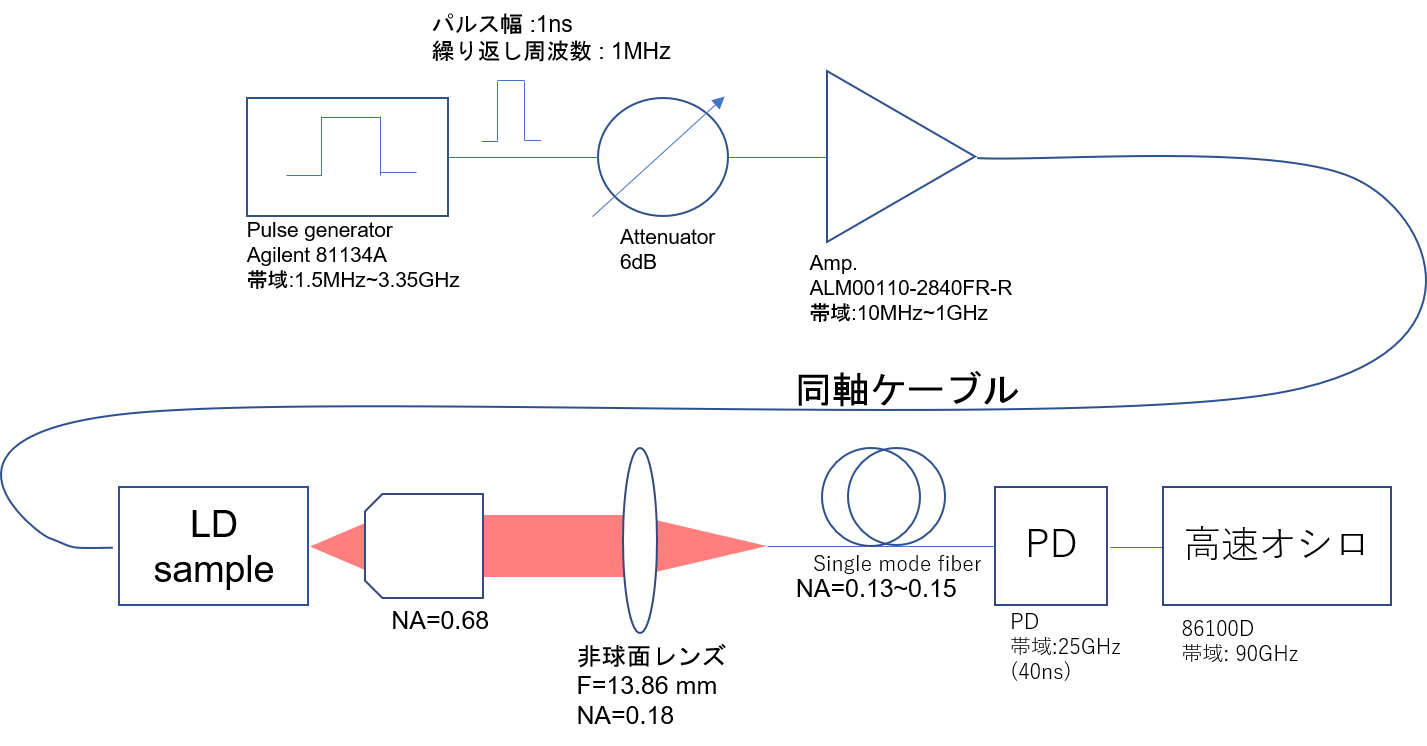
\includegraphics[width=15cm]{figure/fig_2_3_GS_setup.png}
	\caption{GS実験系}
	\label{fig:fig_2_3_GS_setup}
\end{figure}
この実験で用いた機材を表\ref{table:table_2_2_GS_setup}にまとめた。
\begin{table}[hbtp]
  \caption{利得スイッチング実験に用いた機材}
  \label{table:table_2_2_GS_setup}
  \centering
  \begin{tabular}{lcr}
    \hline
    機材  & 型番   & 帯域  \\
    \hline \hline
    Pulse Generator  & Agilent 81143A & 1.5MHz$\sim$ 3.35GHz   \\
    Atteuator  &  埋める    & 埋める\\
    RF Amp & ALM00110-2840FR-R & 10MHz $\sim$ 1GHz \\
    PD & 埋める & 25GHz \\
    Oscilloscope  &  86100D & 90GHz  \\
       \hline
  \end{tabular}
\end{table}
